%% LyX 2.2.3 created this file.  For more info, see http://www.lyx.org/.
%% Do not edit unless you really know what you are doing.
\documentclass[english,nohyper,9pt,A4]{tufte-handout}
\usepackage{fontspec}
\usepackage{unicode-math}
\setmainfont[Ligatures=TeX]{TeX Gyre Bonum}
\setsansfont[Ligatures=TeX]{Marcellus SC}
\setmonofont{Fira Code}
\usepackage{fancyhdr}
\pagestyle{fancy}

\makeatletter

%%%%%%%%%%%%%%%%%%%%%%%%%%%%%% LyX specific LaTeX commands.

\title{\textsf{\textbf{Bound together or loose ends?}}\\
\textsf{\textbf{Foraging association in Red Knots}}}
\author{\textsf{\textsf{Pratik R Gupte}$^{1,2}$, \textsf{Selin Ersoy}$^{1,2}$ \& \textsf{Allert I Bijleveld}$^{2}$}}

%%%%%%%%%%%%%%%%%%%%%%%%%%%%%% Textclass specific LaTeX commands.
\newcommand{\lyxaddress}[1]{
\par {\raggedright #1
\vspace{1.4em}
\noindent\par}
}

\@ifundefined{date}{}{\date{}}
%%%%%%%%%%%%%%%%%%%%%%%%%%%%%% User specified LaTeX commands.
\setmathfont{TeX Gyre Bonum Math}

\makeatother

\usepackage{polyglossia}
\setdefaultlanguage[variant=american]{english}
\begin{document}
\maketitle

\lyxaddress{${^1}$ \textsf{GELIFES --- University of Groningen}\\
${^2}$ \textsf{COS --- NIOZ Netherlands Inst. Sea Research}}

\lyxaddress{\textsf{Contact: p.r.gupte@rug.nl; Twitter: @pratikunterwegs}}

\small

\subsection{Introduction and Methods}

Waders such as red knots \emph{Calidris canutus} are highly social,
and gather in large non-breeding flocks in the Wadden Sea, where they
feed on the macrozoobenthos buried in intertidal mudflats. Knots have
been shown to use social information in lab settings\footnote{Bijleveld et al. 2015.\emph{ Behav. Processes}},
and are hypothesised to use communal roosts as information centres\footnote{Bijleveld et al. 2010.\emph{ Oikos}}.
Persistent association with specific individuals could help knots
make use of collective sensing, or exploit an informed flockmate.
We used high frequency\emph{ (1 minute interval) }ATLAS\footnote{Time of Arrival radio tracking using tags glued to dorsal surface;
5-point median filter applied.} tracking data to test whether knots have non-random associations
— in a sense, do knots have friends?

\subsection{Results}

We found that of 556 unique knot pairs tracked over 44 tidal intervals
\emph{(high tide to high tide, \textasciitilde{}19 days)}, only \textasciitilde{}10\%
had a co-occurence \emph{(proportion of positions in proximity)} higher
than expected by chance. Within tidal intervals, knot co-occurrence
was highest in the hours just before \emph{(advancing tide)} and after
\emph{(receding tide)} high tide, and lowest around low tide (Fig.
1). 

\begin{marginfigure}
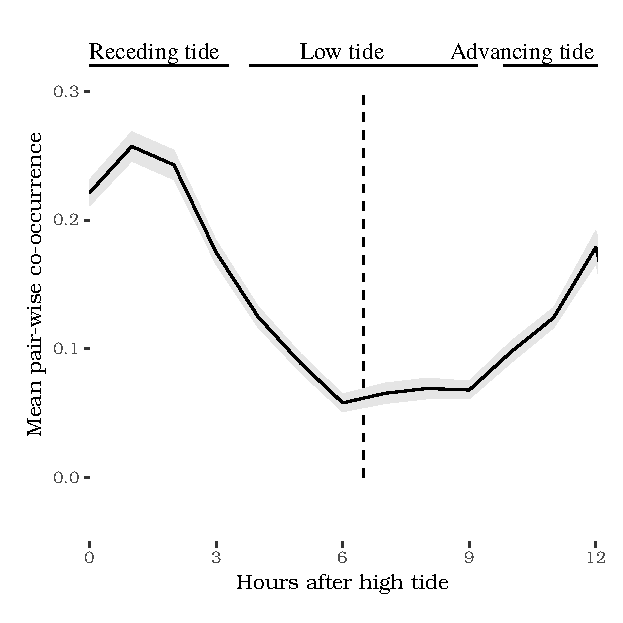
\includegraphics[width=1\textwidth]{/home/pratik/git/knots/knots_code/figure_coherence_hour_handout.eps}
\caption{\emph{Mean pair-wise co-occurrence over the tidal interval ${\pm}$ 95${\%}$ CI. Low tide at dashed line.}}
\end{marginfigure}We further found that the co-occurrence of a pair in the advancing
tide was not related to its co-occurrence prior to the foraging period\emph{,
i.e., }in the receding tide. However, pairs with high co-occurrence
in the advancing tide had travelled similar distances in the foraging
period around low tide.

\subsection{Discussion}

Our results align with the long-held notion that wader flocks are
good examples of random mixing driven by environmental effects\footnote{Myers 1983. \emph{Behav. Ecol. Sociobiol.}; Conklin \& Colwell 2007.
\emph{JOFO.}} — possibly, individual presence is sufficient to inform about the
resource landscape without individual identity being key. Further,
association and information use may occur at a larger or finer scale
than used here\footnote{Harrington \& Leddy 1982. \emph{Wader Study Group Bull.}}.

Red knots have been shown to have consistent individual differences
in exploratory behaviour, which may be linked to different foraging
needs and movement patterns\footnote{Bijleveld et al. 2014. \emph{Proc. Royal Soc. B.}}.
It remains to be tested both whether knots are more discriminating
about the \emph{kind}, rather than identity, of individuals with which
they associate.
\end{document}
